\section{First Experimental Tests}

% I've completely skipped the SLAC experiments from early 1980s E80 and E130.  They used polarized electrons on polarized protons and thus had a  smaller kinematic coverage (no low x data)

In 1988, the European Muon Collaboration (EMC) published data on asymmetries of longitudinally polarized muon beams scattering off of longitudinally polarized proton targets.  The asymmetry they measure is related to the virtual photon asymmetries $A_1$ and $A_2$ as
%
\begin{equation}
  A \equiv \frac{d\sigma^{\uparrow \downarrow} - d\sigma^{\uparrow \uparrow}}{d\sigma^{\uparrow \downarrow} + d\sigma^{\uparrow \uparrow}} = D (A_1 + \eta A_2)
\end{equation}
%
where the coefficients $D$ and $\eta$ can be written in terms of the usual DIS kinematic variables and $R$, the ratio of longitudinal and transverse photoabsorption cross sections:
%
\begin{equation}
  D = \frac{y(2-y)}{y^2 + 2(1-y)(1+R)}, ~~~~~~~~ \eta = \frac{2(1-y)}{y(2-y)} \frac{\sqrt{Q^2}}{E}
\end{equation}
%
Following ?? \cite{??} we can write the asymmetries $A_1$ and $A_2$ in terms of the $g_1$ and $g_2$ stucture functions:
\begin{equation}
  A_1 = \frac{g_1 - \gamma^2 g_2}{F_1}, ~~~~~~~~ A_2 = \frac{\gamma (g_1 + g_2)}{F_1}
\end{equation}
%
where
%
\begin{equation}
  \gamma = \sqrt{\frac{2Mx}{Ey}}
\end{equation}


From these data they extracted measurements of the proton's $g_1$ structure function over a wide range in $x$ and $Q^2$.  As shown in Figure \ref{fig:emc-g1p}, the integral value of $g_1^p$ obtained from that extraction was incompatible with the prediction from Ellis and Jaffe.

% measured asymmetry


\begin{equation}
  A_1 = (g_1 - \gamma^2 g_2)\frac{1}{F_1}, ~~~~~~~~ A_2 = \gamma(g_1+g_2)\frac{1}{F_1}
\end{equation}

\begin{figure}
  \includegraphics[width=1.0\textwidth]{figures/emc-g1p}
  \caption{EMC extraction of $g^1_p$ and its integral compared to the prediction from Ellis-Jaffe \cite{Ashman:1987hv}}
  \label{fig:emc-g1p}
\end{figure}

\begin{equation}
  A_1 \approx \frac{A_{\parallel}}{D} \approx (1 + \gamma^2)\frac{g_1}{F_1}
\end{equation}

EMC measures first moment of g1, taking a3 and a8 from beta-decay measurements means that we can extract a0 from $\Gamma_1^p$ and it's $\sim$ 0.  But

\begin{equation}
  a_0 = \Delta \Sigma = a_8 + 3(\Delta s + \Delta \bar{s})
\end{equation}

from above, and if you ignore strange quark contributions (Ellis-Jaffe) you get $a_0 \sim 0.59$, obviously in stark contrast to EMC.  This is the original ``spin crisis''.  And of course $a_0 = 2<S_z^{quarks}>$.

Any need to mention ``Cloudy Bag'' model here?  I think not.

\begin{figure}
  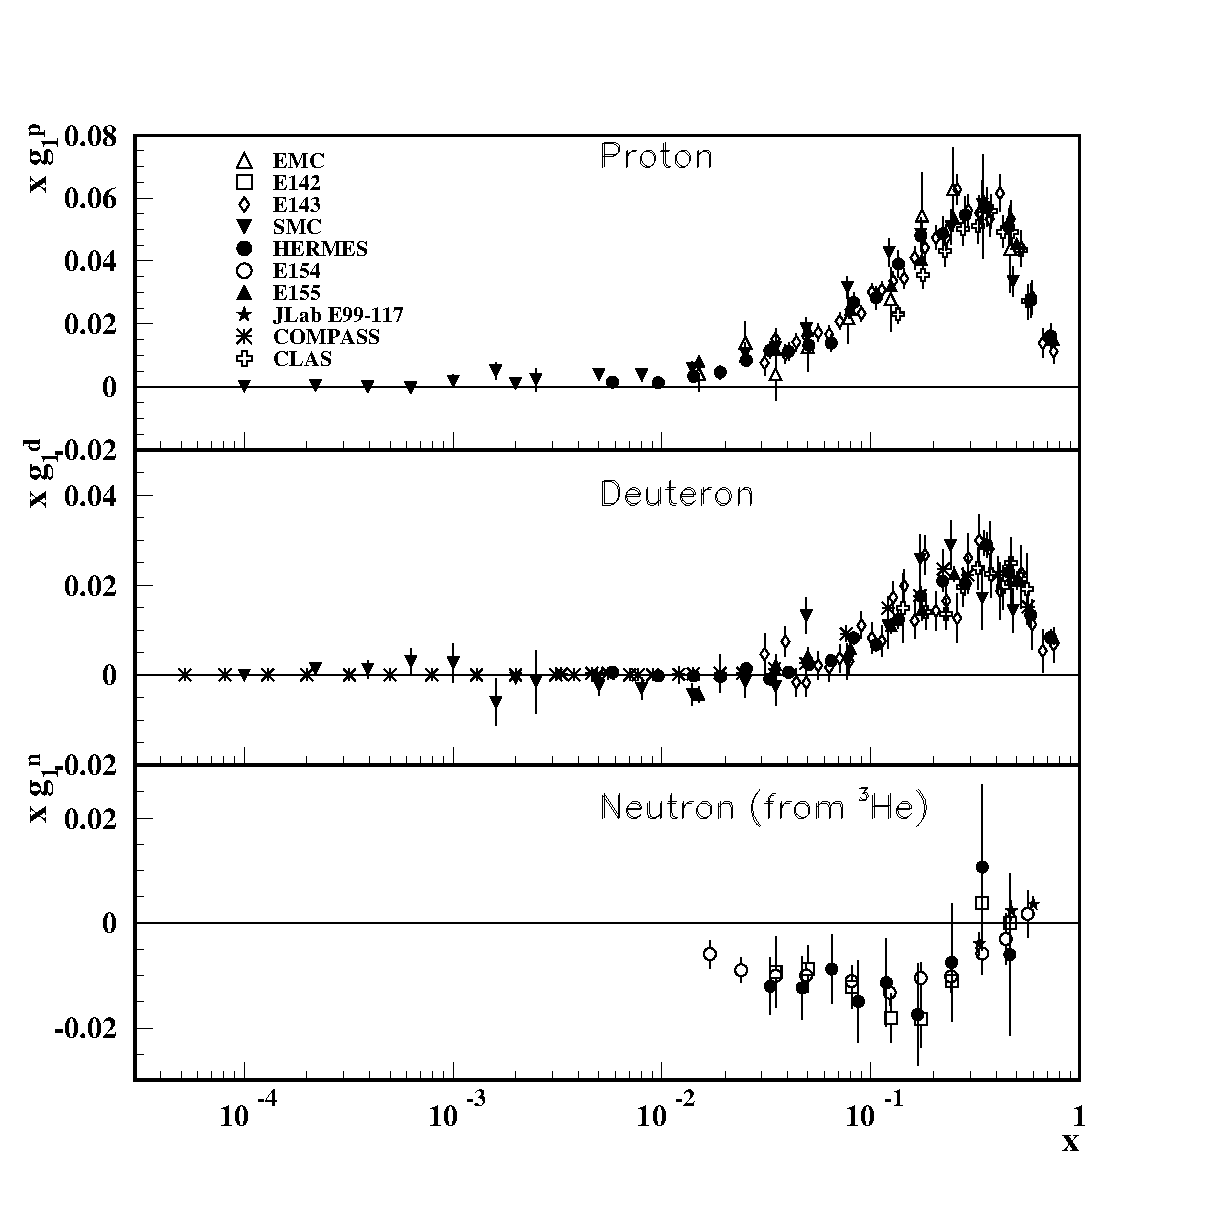
\includegraphics[width=1.0\textwidth]{figures/g1vsx}
  \caption{World data on the $g_1$ structure functions of the proton, neutron, and deuteron \cite{Amsler:2008zzb}}
  \label{fig:g1vsx}
\end{figure}

Detailed derivation of these results can be found in \cite{Anselmino:1994gn}

\begin{equation}
  y \equiv \frac{\nu}{E} = \frac{P \cdot q}{P \cdot k}
\end{equation}

\begin{equation}
  \gamma^2 = \frac{4M^2x^2}{Q^2}
\end{equation}

\begin{equation}
  A_{\parallel} \equiv \frac{d\sigma^{\rightarrow \Leftarrow} - d\sigma^{\rightarrow \Rightarrow}}{2d\sigma_{unpol}}
\end{equation}

\begin{equation}
  A_{\perp} \equiv \frac{d\sigma^{\rightarrow \Uparrow} - d\sigma^{\rightarrow \Downarrow}}{2d\sigma_{unpol}}
\end{equation}